\documentclass[12pt]{article} %amsart documentation:
\usepackage[hmargin=1in, vmargin=1in]{geometry} % Marginshttps://ctan.math.washington.edu/tex-archive/macros/latex/required/amscls/doc/amsclass.pdf
% The Proposal and Award Policies and Procedures Guide
% (PAPPG: https://www.nsf.gov/publications/pub_summ.jsp?ods_key=pappg)
% mandates, in Chapter 2, section B.2, that the main text should have a font size no less
% than 11 points for *most* typefaces (including Computer Modern Roman and Times (new) Roman).
% 
% Actually, Helvetica (a.k.a. Arial), Palatino and Courier New can drop
% to 10 point font size, according to the PAPPG,  but be aware:
% 10-point fonts (whatever the typeface) will promote reader fatigue.
% Reader fatigue never works to the author's advantage.
%
% This sample is set in 12 point type.
%

%choosing fonts: https://www.overleaf.com/learn/latex/Font_typefaces
\fontfamily{cmr}\selectfont %computer modern roman


\usepackage{amsmath,amsthm,amssymb,amscd}
\usepackage[numbers]{natbib}
\usepackage{graphicx}
\usepackage{caption}
\usepackage{subcaption}
\usepackage{wrapfig}

\usepackage{sectsty}
\sectionfont{\fontsize{15}{15}\selectfont}
\subsectionfont{\fontsize{13}{13}\selectfont}


%
%
\renewcommand{\footnotesize}{\small\spaceskip4pt plus1.5pt}

%Pagination - research.gov does this automatically see PAPPG II.B.1
%\advance\footskip1cm %moves footer down on page
\pagenumbering{arabic}
\usepackage{fancyhdr}
\pagestyle{fancy}
\lhead{}
\chead{}
\rhead{}
\lfoot{}
\cfoot{\thepage}
\rfoot{}
\renewcommand{\headrulewidth}{0pt}

\newcommand{\aj}{AJ}
\newcommand{\apj}{ApJ}
\newcommand{\apjl}{apJL}
\newcommand{\apjs}{ApJS}
\newcommand{\aap}{A\&A}
\newcommand{\aaps}{A\&AS}
\newcommand{\araa}{ARAA}
\newcommand{\mnras}{MNRAS}
\newcommand{\baas}{BAAS}
\newcommand{\zap}{ZAP}
\newcommand{\prr}{PRR}
\newcommand{\prf}{PRF}
\newcommand{\sol}{\ensuremath{\odot}}
\newcommand{\RB}{Rayleigh-B\'{e}nard }
\newcommand{\grad}{\ensuremath{\nabla}}

\graphicspath{{./figures/}}

%Make bibliography 2col
\usepackage[normalem]{ulem}
\usepackage{multicol}
\usepackage{enumitem}
\bibliographystyle{apj_small}
\makeatletter
\renewenvironment{thebibliography}[1]
     {\begin{multicols}{2}[\paragraph*{\refname}\vspace{-0.1in}]%
      \@mkboth{\MakeUppercase\refname}{\MakeUppercase\refname}%
      \list{\@biblabel{\@arabic\c@enumiv}}%
           {\settowidth\labelwidth{\@biblabel{#1}}%
            \leftmargin\labelwidth
            \advance\leftmargin\labelsep
            \@openbib@code
            \usecounter{enumiv}%
            \let\p@enumiv\@empty
            \renewcommand\theenumiv{\@arabic\c@enumiv}}%
      \setlength{\itemsep}{-2pt}
      \sloppy
      \clubpenalty4000
      \@clubpenalty \clubpenalty
      \widowpenalty4000%
      \sfcode`\.\@m}
     {\def\@noitemerr
       {\@latex@warning{Empty `thebibliography' environment}}%
      \endlist\end{multicols}}
\makeatother

%PAPPG: https://www.nsf.gov/publications/pub_summ.jsp?ods_key=pappg
\begin{document}
%\thispagestyle{fancy}

\centerline{\bf\large NHFP: Building modern models of convection in massive stars}

\paragraph{Abstract}
Massive stars are the cornerstone of many fields of astrophysics. 
Modern precision observations have revealed major shortcomings in theoretical models of massive stars which demand new prescriptions of convection informed by simulations. 
The research goal of this proposal is to build a next-generation set of 3D numerical simulations of convection in massive stars, which will answer the following questions:
(1) How large are convective cores in massive stars?
(2) How do opacity-driven convective shells affect the structure of massive stars, their position on the HR diagram, and observable waves at the stellar surface?
The proposed host institution is the University of California, Santa Barbara (UCSB), within the Kavli Institute for Theoretical Physics (KITP). 

\setcounter{section}{0}

\section{Summary of Previous and Current Research}
My research is rooted in fluid dynamics and inspired by observations of stars.
I use the \emph{Dedalus} \citep{burns_etal_2020} pseudospectral code to design and run state-of-the-art simulations which I use to learn about mixing processes like convection in stars.
\textbf{A core focus of my research has been to push the boundaries of \emph{time} evolution, while other studies have focused on \emph{spatial} resolution; my focus on the time domain has led to key discoveries in my career.}

For example, as a graduate student, I studied how fast convection interacts with the slow evolution of the background thermal structure in convective regions \citep{anders_etal_2018,anders_etal_2020}; some dynamical snapshots from these studies are shown in Fig.~\ref{fig:past_ae}.
My graduate research also included studies of heat transport in compressible convection with  \citep{anders_etal_2019_rot} and without \citep{anders_brown_2017} rotation.
Finally, as a graduate student I studied convection at the smallest scales, examining individual downflows in the Sun's convection zone \citep{anders_etal_2019_thermals}.

\begin{figure}[b!]
     \centering
     \captionsetup{width=0.97\linewidth}
     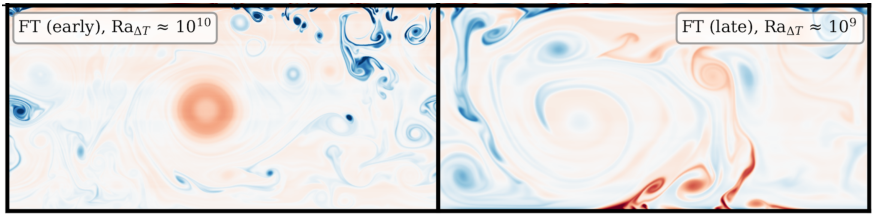
\includegraphics[width=\textwidth]{past_ae.pdf}
        \caption{Snapshots of the temperature anomaly in convective simulations at
early (left) and late (right) times \citep{anders_etal_2020}. 
The disequilibrium early state demonstrates more turbulent flows and flow asymmetries than occur in the evolved, saturated state.
        \label{fig:past_ae}}
\end{figure}

As a postdoctoral fellow at Northwestern, I have connected my theoretical research with modern observational puzzles.
I have formed collaborations with observers and 1D modelers alike to understand what sets the position of a convective boundary \citep{anders_etal_2022b} (see Fig.~\ref{fig:past_cbm}, top panels), and I have discovered the process that inflates the convective cores of stars relative to standard models \citep{anders_etal_2022a} (see Fig.~\ref{fig:past_cbm}, bottom panels).

\begin{figure}[t!]
     \centering
     \captionsetup{width=0.97\linewidth}
     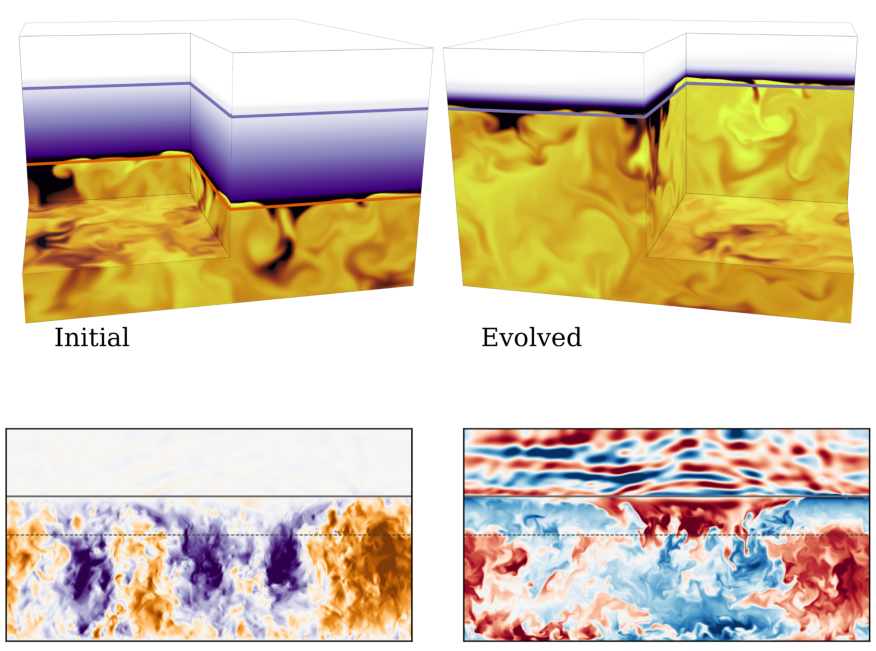
\includegraphics[width=\textwidth]{past_cbm.pdf}
        \caption{
        (Top panels) Snapshots of the composition field in a convective simulation at early (left) and late (right) times \citep{anders_etal_2022b}. 
        The stable composition gradient (purple gradient) is entrained over time by overshooting convective motions into the well-mixed (yellow) convection zone.
        (Bottom panels) Snapshots of the vertical velocity (left) and temperature anomaly (right) at the same time in a simulation with convective penetration \citep{anders_etal_2022a}. 
        In the left panel, we see broad upflows (orange) and downflows (purple). 
        Upflows are hot (red) in the bulk convection zone but turn cold (blue) when they cross into the penetration zone (between the dashed line and solid line).
        \label{fig:past_cbm}}
        \vspace{-0.3cm}
\end{figure}



My current research focuses on interactions between the convective core and the radiative envelope in massive stars.
I am studying the gravity waves in the radiative envelope driven by core convection.
My current research goals are to characterize both the spectrum of waves convection generates and the observable features of these waves after they propagate through the radiative envelope.
I will directly compare the waves in my simulations to asteroseismic observations of waves in massive stars.
As a part of this work, I have developed and tested a preliminary \emph{Dedalus} module which solves the fully compressible equations using a massive star \emph{MESA} model for the background state (Fig.~\ref{fig:star}).
This existing code will allow me to immediately pursue my Focus I tasks (below) upon arriving at KITP, and has provided me with the tools necessary to successfully implement the simulations for Focus II (also below).

\begin{wrapfigure}{r}{0.5\textwidth}
  \begin{center}
      \vspace{-3cm}
    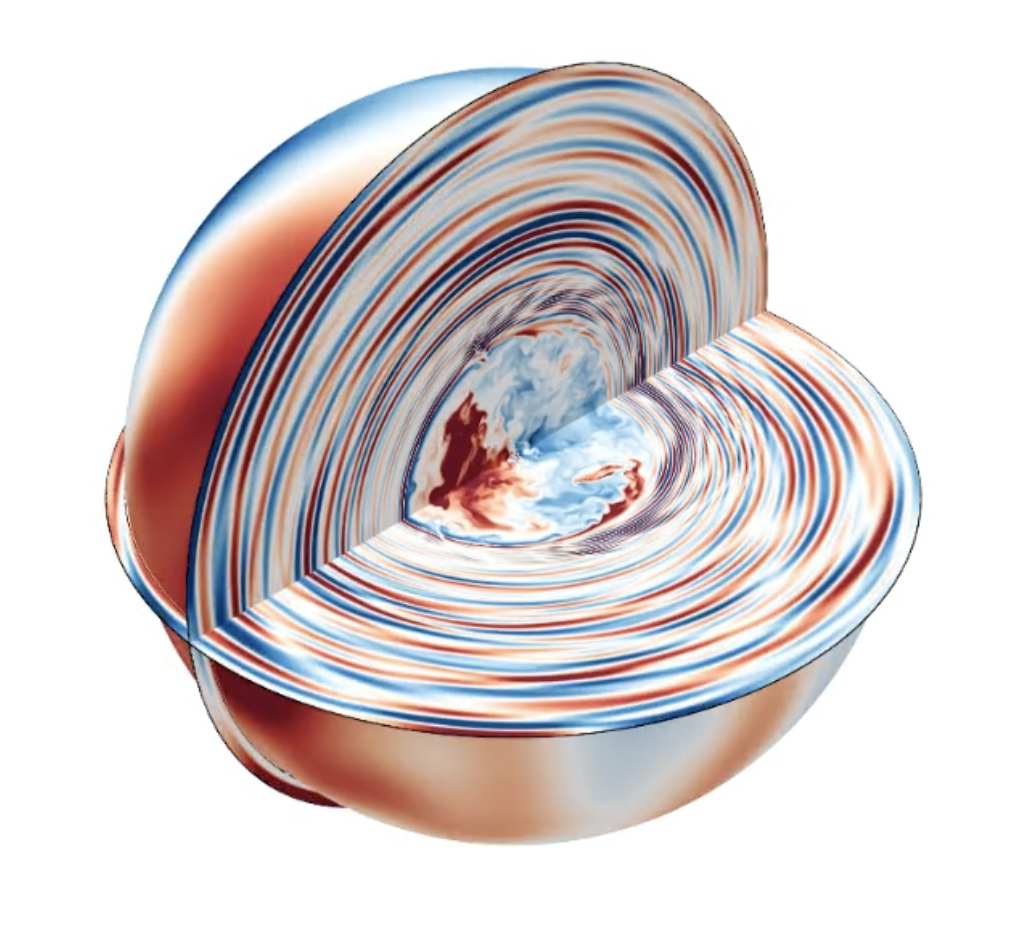
\includegraphics[width=0.45\textwidth]{dedalus_massive_star.png}
      \vspace{-0.8cm}
  \end{center}
    \caption{A simulation I ran in \emph{Dedalus} of a {$40 \,M_{\odot}$} star. 
    The entropy field is visualized; red is hot and buoyantly rises, blue is cold and falls. 
    We see a convective core with a strong dipole flow and an outer radiative envelope with internal gravity waves. \label{fig:star}}
    \vspace{0.0cm}
\end{wrapfigure}

\section{Research Proposal} \vspace{-0.2cm}

\subsection{Motivation} \vspace{-0.15cm}

Massive stars are the cornerstone of many fields of astrophysics.
Ionizing radiation from massive stars was important in the reionization of the early universe \citep{bromm_larson_2004} and regulates both star formation and the interstellar medium structure \citep{lancaster_etal_2021}.
Massive stars end their lives in dynamic explosions which produce supernovae and observable high-energy transients \citep{heger_2003} and leave behind compact remnants like black holes and neutron stars \citep{abbott_etal_2018}.
A star's properties---ranging from its surface radiation field to the type of explosion that ends its life---depend intricately on its complex evolutionary history \citep{farmer_etal_2016}, which involves many uncertainties.
One key source of error in stellar modeling and evolution is the treatment of convection.


\textbf{Modern precision observations have revealed major theoretical shortcomings in models of stars and stellar convection.}
Asteroseismology and eclipsing binary studies reveal the need for larger convective cores than standard models produce \citep{johnston2021}.
Modern spectroscopic and photometric (\emph{Gaia}) observing campaigns have provided exquisitely detailed HR diagrams of stellar clusters, but stellar models do not reproduce the observed populations without adjusting the sizes of convective regions \citep{castro_etal_2014,gaia_2018,martinet_etal_2021}.
Kilometer-scale gravitational wave observatories (e.g., \emph{LIGO}/\emph{VIRGO}) are probing the populations of massive remnants \citep{abbott_etal_2018}, and convective mixing influences theoretical predictions of gaps in the remnant distribution \citep{vanson_etal_2022,farmer_etal_2019}.
Convection is a 3D turbulent process which adjusts a star's thermal structure and efficiently mixes chemical discontinuities, but is typically implemented in stellar evolution models using some form of the decades-old mixing length theory \citep[MLT,][]{bohmvitense_1958}, which has many shortcomings.
%Stellar models cannot explain our modern precision observations, and convection is at the root of many disagreements between models and observations.
\textbf{Disagreements between theory and observations demand new state-of-the-art models of convection informed by 3D simulations. }

The cores of massive stars ($M_* \gtrsim 1.1 M_\odot$) host convection, and the size of the convective core is a key uncertainty in massive star evolution.
Some type of convective boundary mixing (CBM) is often invoked to expand the core size to align 1D models with observations.
For example, in order to reproduce the observed population of eclipsing binaries, stellar models must employ a mass-dependent CBM \citep[see Fig.~\ref{fig:intro}, middle;][]{claret_torres_2019}.
%Apsidal motion in binaries can be used to probe the density structure of stars \citep{rosu_etal_2022}, and these measurements suggest substantial CBM occurs.
When stars in stellar clusters are placed on the HR diagram, we observe wider main sequences than standard evolutionary models predict \citep{castro_etal_2014,higgins_vink_2019}, but introducing a mass-dependent CBM aligns models with observed populations.
Finally, asteroseismology measures the radial profile of mixing processes inside stars; these measurements reveal extensive CBM outside of convective cores \citep{michielsen_etal_2019,pedersen_etal_2021}.
%This body of evidence suggests that additional mixing is required at the core convective boundary of massive stars, but observed mass-dependent trends have no robust theoretical explanation \citep{johnston2021} and CBM is often treated as a free parameter.
Ad-hoc CBM prescriptions used in the literature produce core masses which vary by 70\% \citep{kaiser_etal_2020}, and these prescriptions must be finely tuned to match observations.
Larger convective cores achieved by CBM have access to excess fuel, so it is impossible to accurately predict fundamental stellar properties like the star's lifetime, its pathway through the HR diagram, and the character of the remnant it leaves behind without improved CBM models.
%A unifying theory of CBM which reproduces observations self-consistently based on properties of stellar structure is desired.

\begin{figure}[t!]
     \centering
     \captionsetup{width=0.97\linewidth}
     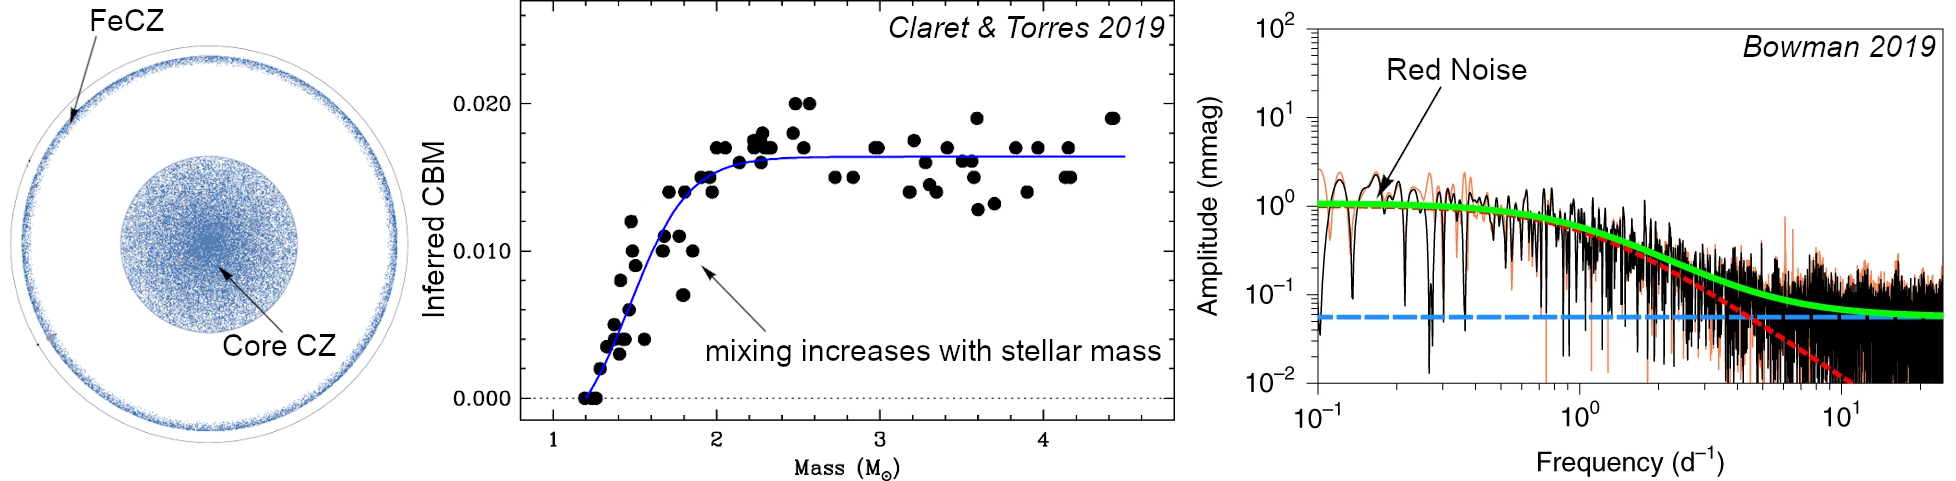
\includegraphics[width=\textwidth]{fig1.png}
        \caption{(Left) The structure of a massive star; shaded regions denote the core convection zone (core CZ) and iron convection zone (FeCZ) \citep{jermyn_etal_2022_atlas}.
        (Middle) Inferred convective mixing (y-axis) versus stellar mass for eclipsing binaries; note the strong mass dependence \citep{claret_torres_2019}.
        (Right) An amplitude spectrum of ``red noise'' in a hot, massive star; note the appreciable signal (black line) in excess of the noise floor (blue line) at low frequencies \citep{bowman_etal_2019}. 
        \label{fig:intro}}
\end{figure}

The surfaces of massive stars are dynamic.
Motions at the stellar surface broaden spectral lines in a phenomenon generally referred to as ``macroturbulence'' \citep{schultz_etal_2022b}.
A recent study of hot massive stars has also revealed a flat excess of power or ``red noise'' at low temporal frequencies \citep[see Fig.~\ref{fig:intro}, right;][]{bowman_etal_2019}.
%Until recently, it was believed that the only convective engine in massive stars was the core convection zone (core CZ), but updates in opacity tables have revealed that massive stars have more convection zones than previously thought .
In addition to core CZs, most massive stars have opacity-driven convective shells near their surfaces introduced by specific ionization states of hydrogen, helium, and iron \citep[see Fig.~\ref{fig:intro}, left;][]{cantiello_etal_2009}.
The ``iron-bump'' convection zone (FeCZ) is of particular interest.
Turbulent motions in FeCZs could produce macroturbulence and red noise \citep{cantiello_etal_2021, schultz_etal_2022, schultz_etal_2022b}.
Only a few simulations of FeCZs exist \citep{jiang_etal_2015}, so it is still unclear whether e.g., red noise is a manifestations of core gravity waves---in which case it can be used to probe stellar structure---or a manifestations of FeCZ turbulence.
In addition to producing poorly characterized turbulent dynamics, FeCZs are highly radiation-dominated and the luminosity typically approaches the Eddington limit \citep{jermyn_etal_2022_atlas}.
In this extreme regime, standard stellar models produce density inversions which require ad-hoc solutions to stably evolve stellar evolution models \citep{kohler_etal_2015}.
These effects combine to inflate the stellar radius, which in turn reduces the effective surface temperature; the effective temperature is a fundamental input to wind-driven mass loss prescriptions \citep{yusof_etal_2013}.
The presence of an FeCZ therefore introduces uncertainty both into the thermal structure of a star and its mass loss history, which in turn affect the star's evolutionary track and remnant formation processes in a similar but orthogonal manner to core CZ CBM.

These puzzles demand models that go beyond the current state-of-the-art.
\textbf{The goal of this proposal is to build a next-generation set of 3D numerical simulations of convection in massive stars, which will answer the following questions:}
\begin{enumerate}
    \item How large are convective cores in massive stars?
    \item How do opacity-driven convective shells affect the structure of massive stars, their position on the HR diagram, and observable waves at the stellar surface?
\end{enumerate}

\subsection{Focus I: Convective Boundary Mixing} \vspace{-0.15cm}
Observations require improved models of convective boundary mixing (CBM) \citep{johnston2021}.
I recently produced simulations which demonstrated that energetically equilibrated convection zones can expand beyond the Schwarzschild boundary \citep[Fig.~\ref{fig:past_cbm}, bottom panels;][]{anders_etal_2022a}.
These simulations used approximations (Cartesian geometry, incompressible flows) which are not valid within the cores of massive stars.
Despite their simplicity, a CBM prescription calibrated using my simulations self-consistently reproduces many characteristics of observed CBM trends \citep{jermyn_etal_2022_penconv}.
This promising preliminary alignment between my theoretical work and observations demands a calibrated prescription from more realistic simulations.

Stellar core convection is difficult to simulate.
Many codes mathematically require a ``cutout'' near $r = 0$, so flows cannot pass through the center of the star \citep{edelmann_etal_2019,horst_etal_2020,yadav_etal_2016}.
Core convection also occurs at very low Mach numbers \citep[Mach $\sim 10^{-4}$;][]{jermyn_etal_2022_atlas,aerts_etal_2021}, and standard explicit timestepping techniques must use very small timesteps to resolve the (fast) sound waves \citep{edelmann_etal_2021}. 
Past studies have avoided timestepping restrictions by employing the Anelastic approximation \citep[thermodynamically invalid for CBM studies;][]{brown_etal_2012,browning_2008,yadav_etal_2016} or by boosting the stellar luminosity \citep[which leads to unphysical excess CBM;][]{baraffe_etal_2021}.

I will address these modeling deficiencies by simulating core convection in massive stars using the \emph{Dedalus} \citep{burns_etal_2020} code.
My simulations will differ from past simulations, because (1) I will include the full ``ball'' geometry of the convective core including $r = 0$, (2) I will not boost the luminosity, and (3) my simulations will be thermally equilibrated.
\emph{Dedalus} has the state-of-the-art ability to simulate flows that pass through the coordinate singularity at $r = 0$ in spherical coordinates \citep[Fig.~\ref{fig:star}; see also Refs.~][]{vasil_etal_2019,lecoanet_etal_2019}.
I have simulated very low Mach number flows without extreme timestep restrictions in \emph{Dedalus} using implicit-explicit (IMEX) timestepping techniques  \citep{anders_brown_2017}, and I will apply these techniques to realistic low-Mach core convection to avoid luminosity boosting.
I have also developed methods of ``accelerated evolution'' \citep{anders_etal_2018,anders_etal_2020,anders_etal_2022a}; these techniques rapidly equilibrate simulations while saving up to an order of magnitude in computational resources, and I will apply these techniques to my simulations to rapidly achieve saturated CBM zones.

Massive stars rotate rapidly \citep{jermyn_etal_2022_atlas}, but CBM studies have neglected rotation because the parameter space of rotating convection is difficult to navigate.
The \emph{Rossby number} (the ratio of the rotational and convective timescales) determines how rotation affects convective flows \citep{aurnou_etal_2020}, but it cannot be determined \emph{a-priori} just by specifying an observationally-based relationship for the stellar rotation rate \citep{glebocki_gnacinski_2005,ramirezagudelo_etal_2013,nielsen_etal_2013}.
I have determined how to navigate the parameter space of rotating convection \citep{anders_etal_2019_rot}, and will study realistic rotating core convection after establishing a non-rotating benchmark.

\emph{\underline{Task 1:}}
I will study CBM in spherical simulations based on \emph{MESA} models of massive stars (as in Fig.~\ref{fig:star}).
In this first task, I will focus on simulations of non-rotating stars spanning the mass range $M_* = 1.1-40 M_{\odot}$.
I will focus specifically on stars from $1.1-3 M_{\odot}$, where observed ``extra mixing'' is a strong function of stellar mass \citep[][Fig.~\ref{fig:intro}, middle]{claret_torres_2019}.

\emph{\underline{Task 2:}} I will study how rotation affects CBM.
Rotation is theorized to reduce the extent of CBM \citep{augustson_mathis_2019}.
In our current theory of CBM via convective penetration \citep{anders_etal_2022a}, the mixing region's size decreases as the dissipation in the convection zone increases.
Rotation organizes flows into highly-dissipative vortices aligned with the rotation axis \citep{julien_etal_1996}, so it makes sense for rotation to decrease CBM, but I will test this explicitly.

\textbf{\underline{\emph{Deliverable:}} The first 3D simulations of rotating core convection in massive stars which include $\boldsymbol{r = 0}$, reach thermal equilibrium, do not boost the luminosity, and span the main sequence.}
These models will inform a 1D prescription of CBM, which I will implement in the 1D \emph{MESA} stellar evolution software instrument.
I will publish the \emph{Dedalus} module used to create these simulations on Github and Zenodo, giving the community an open-source tool for studying dynamics in massive stars. 




\subsection{Focus II: Optically Thick Iron-bump Convection} \vspace{-0.15cm}
%%%%%%%%%%%%%%%%%%%%%%%%%%%%%%%%%%%%%%%%%%%%%%%%%%%%%%%%%%%%%%%%%%%%%%
In addition to vigorous core convection, massive stars have near-surface opacity-driven convective shells \citep{cantiello_etal_2009}.
Iron opacity generates an ``Iron-Bump Convection Zone'' (FeCZ) in stars with masses $\gtrsim 8 M_{\odot}$.
Unlike the photospheric convection zones of lower-mass stars (e.g., the Sun), FeCZs occur in fully optically-thick regions of the star \citep{jermyn_etal_2022_atlas}.
FeCZs can produce extreme dynamics which influence the stellar structure and evolution appreciably \citep{schultz_etal_2022b}.

FeCZs have been simulated in 40 and 80 $M_{\odot}$ stars \citep{jiang_etal_2015}.
Follow-up investigations of these simulations  \citep{schultz_etal_2020,schultz_etal_2022,schultz_etal_2022b} revealed that the high-Mach number FeCZ convection creates a large dynamic pressure which is not included in stellar evolution models.
This turbulent pressure modifies the stellar stratification and alters the effective temperature at the stellar photosphere and should be parameterized and included in 1D evolutionary calculations.
Unfortunately, full radiative hydrodynamical simulations of FeCZs \citep{jiang_etal_2015} are too expensive to produce \emph{en masse} to calibrate a turbulent pressure prescription across the main sequence.

Fortunately, since FeCZs typically occur in optically thick layers \citep{jermyn_etal_2022_atlas}, the computationally-inexpensive radiative diffusion approximation is valid.
Furthermore, FeCZs are very thin and can be accurately studied in plane-parallel Cartesian domains \citep{jermyn_etal_2022_atlas}.
I will extend my prior high-Mach number \emph{Dedalus} convection simulations \citep{anders_brown_2017} by including iron bump opacity effects in the radiative diffusion limit.
I will study FeCZs in stars whose masses span $8-60\, M_{\odot}$ and with ages ranging from the zero-age main sequence (ZAMS) to the terminal age main sequence (TAMS) to calibrate the turbulent pressure generated in FeCZs.

There is a current debate about whether ``red noise'' on hot, massive stars \citep[Fig.~\ref{fig:intro}, right;][]{bowman_etal_2019} is produced by gravity waves generated in the convective core or FeCZ turbulence \citep{cantiello_etal_2021}.
FeCZ simulations produce turbulence which could explain \emph{both} red noise and observed ``macroturbulence'' \citep{schultz_etal_2022,schultz_etal_2022b}.
Simulations of core-generated gravity waves \citep{edelmann_etal_2019,horst_etal_2020} have also shown signals similar to red noise, but do not include the FeCZ, and so do not capture how the FeCZ modifies gravity wave signals from the core.
I will study how gravity wave signals generated below the FeCZ change as they pass through this turbulent convection zone.
%

\emph{\underline{Task 3:}} I will use \emph{Dedalus} to study iron-bump convection in Cartesian, optically thick simulations which span many stellar masses and ages.
I will measure the turbulent pressure and parameterize it for inclusion in \emph{MESA}.
I will work with experts in the \emph{MESA} community to include turbulent pressure into stellar evolution models, then I will generate a new suite of stellar evolution models to quantify how turbulent pressure affects the stellar radius, effective temperature, and other observable properties of these stars.

\emph{\underline{Task 4:}} I will use \emph{Dedalus} to simulate how an FeCZ modifies gravity waves generated by core convection.
I will force a spectrum of gravity waves below the FeCZ, then measure how these waves interact with and are modified by the turbulent convection.
These simulations will put the first constraints on whether or not gravity waves can pass through the FeCZ to be observable at the stellar surface.
Since gravity waves are one of the best tools for putting constraints on the interior structure of massive stars \citep{aerts2010}, it is critical to understand whether their signal is modified or blocked by FeCZs.
%The results of these simulations will help determine whether observers should look towards lower-metallicity, lower-mass stars where there are no opacity-driven convection zones for wave signals \citep{jermyn_etal_2022_window}.

\textbf{\underline{\emph{Deliverable:}} The first 3D simulations of iron-bump convection spanning the HR diagram, and the first 3D calibration of how the FeCZ affects asteroseismic gravity wave observations.}
I will also create a 1D implementation of turbulent pressure, which will improve stellar structure models of massive stars.
As with tasks 1-2, the code used to create these FeCZ simulations will be open-source, published, and widely accessible.


%%%%%%%%%%%%%%%%%%%%%%%%%%%%%%%%%%%%%%%%%%%%%%%%%%%%%%%%%%%%%%%%%%%%%%
\subsection{Timeline \& Feasibility} \vspace{-0.15cm}
Focus I and Focus II are independent and can be studied in parallel.
I will begin work on Focus I in September 2023 and should complete science goals by summer 2025.
I will begin work on Focus II in Spring 2024 and will complete science goals by the end of the fellowship in 2026.
My prior work on coding simulations of stars in \emph{Dedalus} (Fig.~\ref{fig:star}) will let me make progress on Task I immediately upon my arrival at KITP in fall 2023.
The research proposed here should result in at least four papers (two per focus, one per task), as well as open source community \emph{Dedalus} modules for simulating both spherical core convection and thin FeCZ convection (in Cartesian).

From past experience, each of the proposed simulations will cost $\mathcal{O}(10^{4-5})$ cpu-hours, and I will perform $\mathcal{O}(10^{1-2})$ simulations per study, so I will need access to an allocation of $10^{6-7}$ cpu-hours (1-10 million).
I will work with Prof.~Bildsten and UCSB's IT department to acquire this time through UCSB resources (e.g., the SDSC supercomputing center).
If the NHFP makes NASA's HEC program available to me, I will request any additional computing time necessary through NAS machines like \emph{Pleiades} which I have used throughout my career.
Otherwise, I will request NSF ACCESS resources on machines like \emph{Stampede2}. 

\subsection{Relevance to NASA Astrophysics \& Justification of institute} \vspace{-0.15cm}
The proposed research fits under NASA's big question, ``How did we get here?''
This work will improve evolutionary models of massive stars, and these improved models will help us better understand the origin and evolution of the galaxies that make up our universe.
This work will also help answer two fundamental questions posed in the Astro2020 Decadal review: ``What [is] the mass ... distribution of neutron stars and stellar mass black holes?'' and ``What are the most extreme stars and stellar populations?''
The mass of compact objects is one of their fundamental measurable properties, and stellar models provide theoretical constraints on expectations for observed mass distributions.
This work will reduce error in core mixing prescriptions in stellar models, which can lead to errors in core mass estimates of order 70\% \citep{kaiser_etal_2020}.
The proposed FeCZ simulations will lead to better estimates of stellar surface temperature thereby improving estimates of wind-driven mass loss.
CBM errors and mass loss uncertainty affect our ability to determine whether there is mass gap between black holes and neutron stars \citep{vanson_etal_2022} or where the boundaries of the pair instability black hole mass gap lie \citep{farmer_etal_2019}.

UCSB is the ideal location for me to pursue the proposed research.
My expertise on convection and convective boundary mixing---combined with the expertise of my proposed scientific mentor, Prof.~Lars Bildsten, on stellar structure, stellar evolution, and opacity-driven convection---will ensure the success of the critical and timely simulations proposed here.
At UCSB, KITP's scientific programs bring experts to UCSB and KITP with whom I can collaborate on these problems or identify new compelling research questions.
In particular, the announced ``Turbulence in Astrophysical Environments'' program in early 2024 and the ``Interconnections between the Physics of Plasmas and Self-gravitating Systems'' program in summer 2024 can provide beneficial connections for this work.

\vspace{-0.5cm}
\bibliography{biblio.bib}

\end{document}